\documentclass[DM,lsstdraft,toc]{lsstdoc}

\usepackage[english]{babel}
\usepackage[utf8x]{inputenc}
\usepackage{amsmath}
\usepackage{graphicx}
\usepackage{longtable}
\usepackage{hyperref}
\usepackage{comment}
\usepackage{natbib}

\excludecomment{changelog}
\excludecomment{todo}
\excludecomment{openissues}

% Local commands go here
\newcommand{\G}[1]{{\color{green} #1}}
\newcommand{\B}[1]{{\color{blue} #1}}
\newcommand{\R}[1]{{\color{red} #1}}

%% Journal abbreviations
\bibliographystyle{aasjournal}

\title[LSST Science Platform]{LSST Science Platform Vision Document}

\author{
M.~Juri\'c,
D.~Ciardi,
and
G.P.~Dubois-Felsmann
}

\setDocRef{LDM-nnn}
\date{\today}
\setDocRevision{1.0}
\setDocStatus{draft}

\setDocAbstract{%

This document defines the high-level vision for the {\bf LSST Science
Platform (LSP)}, a set of web applications and services through which the
the scientific community will to access, visualize, interact with,
and analyze LSST data holdings.
\\

It is meant to inform the development of requirements, product specifications,
prioritization, and plans for the elements of the DM system that together comprise
the LSP.

}

% Change history defined here. Will be inserted into
% correct place with \maketitle
% OLDEST FIRST: VERSION, DATE, DESCRIPTION, OWNER NAME
\setDocChangeRecord{%
\addtohist{1}{2017-03-15}{Initial high-level description of the concept}{Mario Juric}
%\addtohist{2}{yyyy-mm-dd}{Future changes}{Future person}
}

\begin{document}

% Create the title page
% Table of contents will be added automatically if "toc" class option
% is used.
\maketitle

\section{Preface}

The purpose of this document is to lay out the high-level vision for the {\bf LSST Science Platform (LSP)}, a set of web applications and services through which the the scientific community will to access, visualize, interact with, and analyze LSST data holdings. With its companion document -- the Data Products Definition Document (\DPDD) -- it defines the high-level vision for LSST's end-user deliverables.
\\

To a future LSST user, this document should illustrate what will be made available to the science community through the LSST Data Access Centers. To LSST builders, it provides direction on how to flow down the LSST System Requirements Document to system design, sizing, budget and schedule as they pertain to the end-user services provided at the LSST Data Access Centers.
\\

Though under strict change control\footnote{LSST Docushare handle for this document is {\tt LSE-XXX}.}, this is a {\bf \em living document}. LSST will undergo a period of construction  and commissioning lasting no less than seven years, followed by a decade of survey operations. To ensure their continued scientific adequacy, the high-level vision for LSST Science Platform will be periodically reviewed and updated.

\clearpage

\section{Introduction}

\subsection{Goals and Philosophy}

The LSST is a facility whose primary mission is to acquire, process, and
make available the data collected by its telescope and camera, as well as
enable ``next-to-the-data'' creation of added-value (Level 3) data products
\cite{SRD}.

This document describes the vision for the services to be put into place to
fulfill the ``{\em making available}'' and ``{\em Level 3} creation``
aspects of LSST's mission; its aim is to present a high-level
description of the data access and analysis services provided at the
LSST Data Access Centers.

\subsection{LSST Science Platform Overview}

\begin{figure}
\centering
\scalebox{0.4}{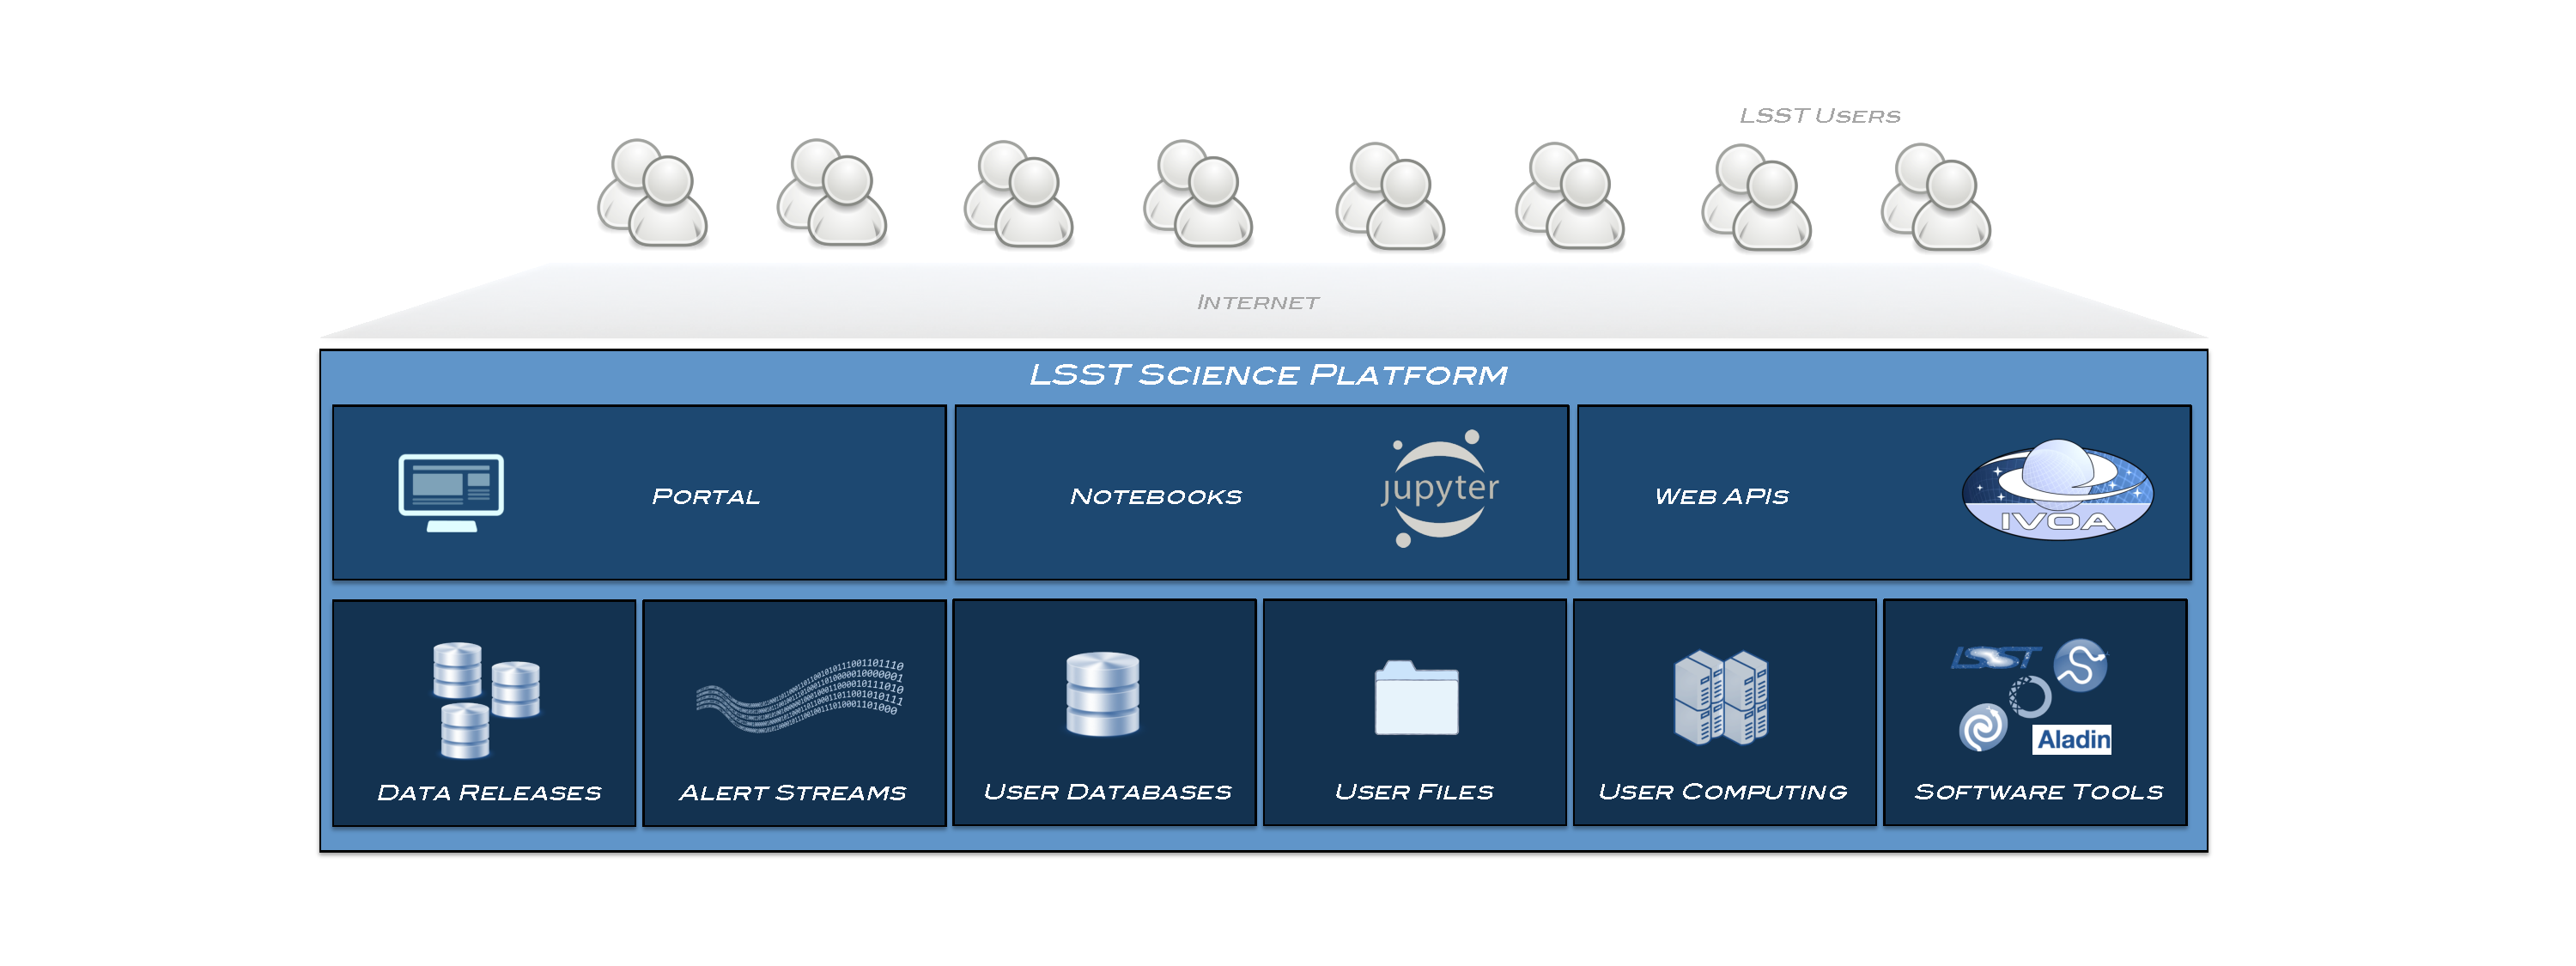
\includegraphics[trim={5cm 0.5cm 3cm 0.5cm},clip,page=1]{images/fig-lsst-science-platform-extended.pdf}}
\caption{
A high-level, layered, view of the LSST Science Platform.  The LSST data
will be exposed to the users through the web Portal, the Jupyter Notebook
interface, and machine-accessible Web APIs.  The web Portal component will
provide the essential data access and visualization services common to
present day archives.  The Notebook component, based on the Jupyter family
of technologies (JupyterHub and JupyterLab) will allow for more
sophisticated next-to-the-data analysis.  These user-visible services will
provide acces to the underlying core LSST data sets -- the data releases and
alert streams -- and be supported by the user Database, File Storage,
Computing, and Software Tools components.  Together, they will enable the
users to access, sub-select, analyze, and perform added-value processing of
all flavors of LSST Data Products (see text for detail). 
\label{fig:layeredLSP}}
\end{figure}

We define the {\bf LSST Science Platform as a set of web applications and services
made available to the scientific community to access, visualize, subset, and
perform next-to-the-data analysis of the LSST data set.}  The platform exposes the LSST data
and services to the user through three primary user-facing {\it aspects} -- the web {\bf Portal},
the {\bf JupyterLab} analysis environment, and a machine-accessible {\bf Web API} interface. These aspects provide three different way to access the data sets and analysis services provided in the LSST Data Access Centers (Figure~\ref{fig:layeredLSP}).

The {\bf Portal} aspect is a web portal designed to provide the essential data
access and visualization services through a simple-to-use website.  It will
enable browsing and visualization of the available datasets in ways the
users are accustomed to at archives such as IRSA, MAST, or the SDSS archive.

The {\bf JupyterLab} aspect will provide a Jupiter Notebook-like interface, and 
is geared towards enabling next-to-the-data analysis. The user experience will 
be nearly identical to working with Jupyter notebooks locally, except that computation
and analysis will occur at resources provided at the LSST Data Access Center.  This is an
implementation of the “bringing computation to the data” paradigm: rather
than imposing the burden of downloading, storing, and processing (large)
subsets of LSST data at their home institutions, we will enable our users to
bring their codes and perform their analysis at the LSST DAC.  We expect
this will reduce the barrier to entry and shorten the path to science for
the LSST science community.

The third, {\bf Web API}, aspect of the LSST Science Platform will expose the
services offered by the LSST Data Access Centers to other software tools and
services using commonly accepted protocols (e.g. industry-standard protocols
such as WebDAV, or Virtual Observatory protocols such as TAP or SIAP). This
interface will open the possibility for remote access and analysis of the LSST 
data set using well-known applications such as TOPCAT or libraries like AstroPy.

Finally, the LSST Science Platform is being envisioned to enable and encourage
collaborative work.  The capabilities ranging from sharing of derived
datasets within smaller groups, collaborations, or with the broader LSST
community, to collaborative visualization and editing capabilities expected
to become available within the JupyterLab ecosystem.

\section{Enabling Remote Data Access and Analysis}

\subsection{Web Portal}

\begin{figure}
	\centering
	\scalebox{0.4}{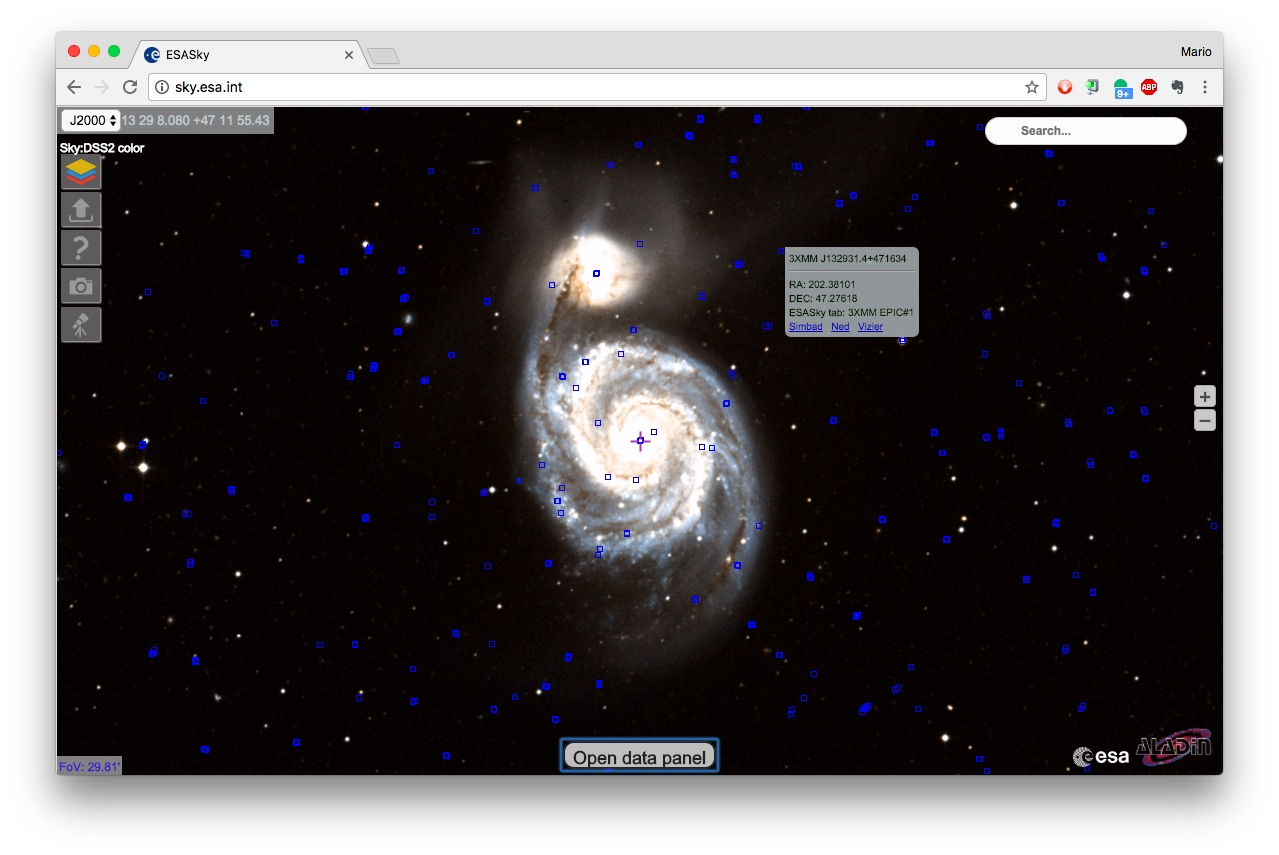
\includegraphics{images/fig-portal-esasky}}
	\caption{The "ESA Sky" web portal interface to ESA Archive holdings. The LSST portal user
		experience will support similar modern pan/zoom/select metaphor for exploration and visualization of the LSST data set.
		\label{fig:portalESA}}
\end{figure}

\begin{figure}
	\centering
	\scalebox{0.4}{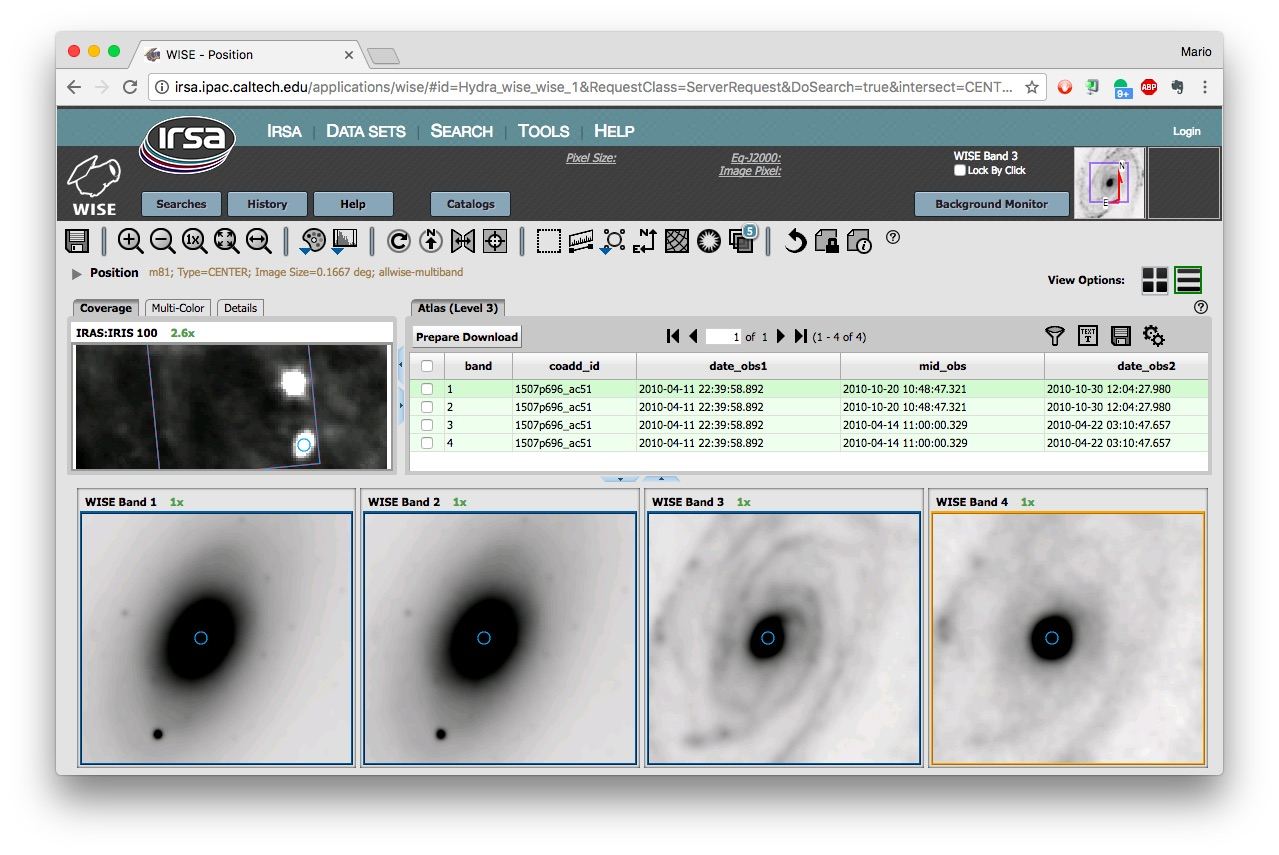
\includegraphics{images/fig-portal-irsa}}
	\caption{The web portal interface to the WISE data set at the Infra-Red Science Archive at IPAC. The LSST portal is being built by extending the Firefly toolkit that powers the IRSA/WISE archive.
		\label{fig:portalIRSA}}
\end{figure}

The {\bf Portal} aspect is a web portal designed to provide the essential data
access and visualization services through a simple-to-use website.  It will
enable browsing and visualization of the available datasets in ways the
users are accustomed to at archives such as IRSA, MAST, or the SDSS archive,
with an enhanced level of interactivity in line with expectations for
then-contemporary archive portals (similar to that found in ESASky and 
the DECaLS Viewer). Examples of the types of user experiences to be offered
through the LSST portal are shown in Figures~\ref{fig:portalESA}~and~\ref{fig:portalIRSA}.

Through the Portal, the users will be
able to view the LSST images, request subsets of data (via simple forms or
SQL queries), store the results of such queries to their personal
workspaces, construct commonly requested plots, and generally explore the
LSST dataset in a way that allows them to identify and access (subsets of)
data required by their science case.

\subsection{JupyterLab}

\begin{figure}
	\centering
	\scalebox{0.4}{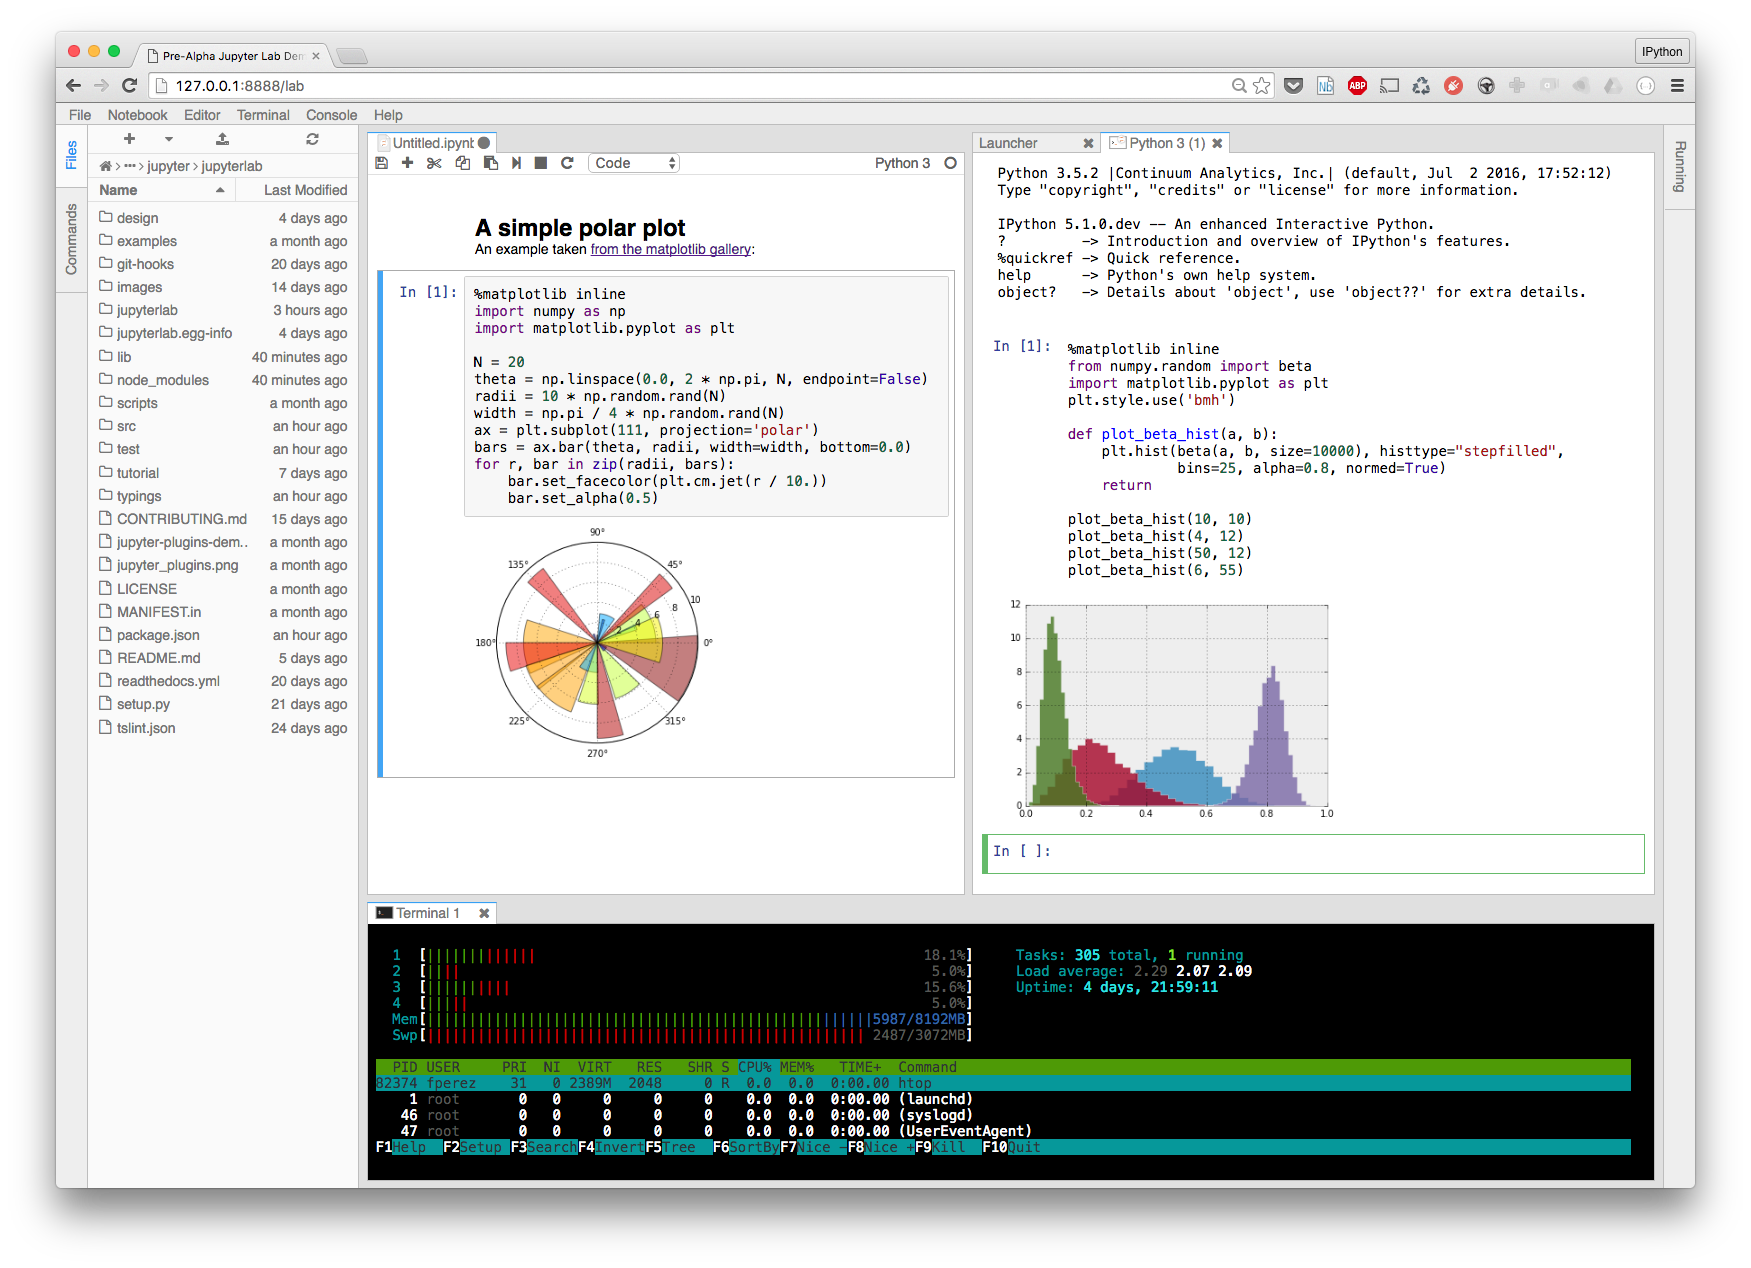
\includegraphics[scale=0.7]{images/jlab-screenshot-nb-con-term-2}}
	\caption{A screen capture of the JupyterLab interface (credit: JupyterLab team, \url{http://blog.jupyter.org/2016/07/14/jupyter-lab-alpha/})
		\label{fig:JupyterLab}}
\end{figure}

The {\bf JupyterLab} aspect, based on the Jupyter family of technologies (such as
JupyterHub and JupyterLab), will be provided to allow for more sophisticated
data selection, analysis, and creation of added value (Level 3) data
products. A screen capture of a mature prototype of JupterLab is shown in 
Figure~\ref{fig:JupyterLab}.

This environment will come preinstalled with a library of
commonly used and useful software Tools (such as AstroPy, LSST software
stack, Anaconda Scientific Python Distribution, and others).  The users will
be able to upload and install their own tools as well.

The JupyterLab user experience will be nearly identical to working with
Jupyter notebooks locally, except that computation and analysis will occur
at resources provided at the LSST Data Access Center.  This is an
implementation of the “bringing analysis to the data” paradigm: rather
than imposing the burden of downloading, storing, and processing (large)
subsets of LSST data at their home institutions, we will enable our users to
bring their codes and perform their analysis at the LSST DAC.  We expect
this will reduce the barrier to entry and shorten the path to science for
the LSST science community.

\subsection{Web APIs}

Backend Science Platform services (including access to
databases, images, and other files) will be exposed through
machine-accessible web APIs serving community-accepted formats and
protocols.  This will make it easy to initiate remote computations operating
on LSST data.  Virtual Observatory interfaces will allow connection to other
archives and enable the use of standard tools such as TOPCAT or DS9. 
This will further lower the barrier to access to LSST data, shortening the
path to science.

\begin{figure}
	\centering
	\scalebox{0.4}{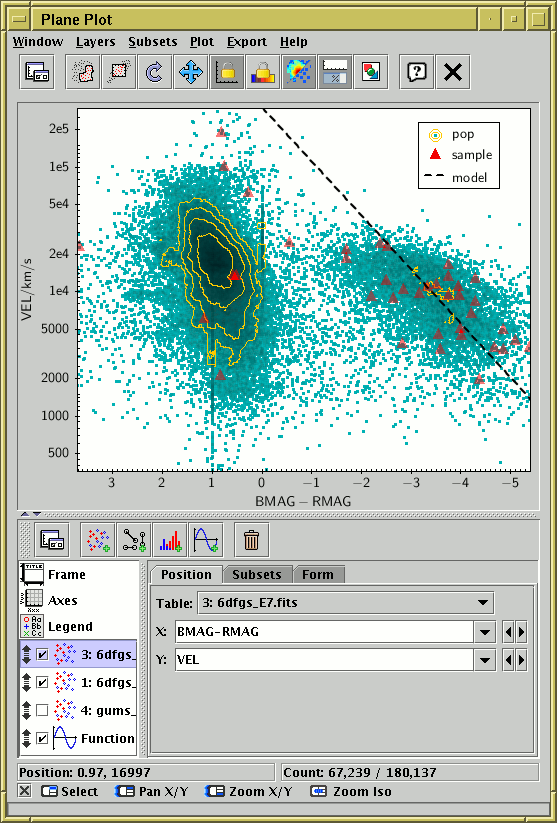
\includegraphics[scale=0.7]{images/topcat-StackPlotWindow}}
	\caption{A screen capture of Tool for OPerations on Catalogues And Tables (TOPCAT), that is capable of remotely accessing catalogs and images using VO protocols. Tools such as these will be able to directly access the data sets served by the LSST DACs (figure credit: Mark Taylor, \url{http://www.star.bris.ac.uk/~mbt/topcat/sun253/sun253.html}).
		\label{fig:toolsTOPCAT}}
\end{figure}

\section{Serving Level 1 and 2: Database and Alert Filtering Services}

All data products will be made available using user-friendly databases and web services. In this section, we describe the high-level concepts for services used to serve the LSST catalogs and the event alert stream. Further details of the LSST data products may be found in the LSST Data Products Definition Document (\DPDD).

\subsection{Serving Catalog Holdings: Relational Databases}

Catalogs are the primary and most frequently used of all LSST data products. Based on surveying the community

To decide which technology best fits the LSST requirements, we did an extensive market research and analyses, reviewed relevant literature, and run appropriate stress-tests for selected “promising” candidates, focusing on weak points and the most uncertain aspects. Market research and analyses involved (a) discussions about lessons learned with many industrial and scientific users dealing with large data sets, (b) discussions about existing solutions and future product road-maps with leading solution providers and promising start-ups, and (c), research road-map with leading database researchers from academia. See 16   Appendix E: People/Communities We Talked To.

\subsection{Alert Filtering Services}

A major Level 1 product of the LSST will be a stream of {\em Event Alerts}, notifications to changes in astrophysical scenery discovered by differencing incoming images against older, deeper, images of the sky in the same direction. These alerts are expected to be numerous --  approaching 10 thousand per visit, totaling 10 million per night -- and transmitted promptly -- with new alerts broadcast within only a minute after observation. More details about event alerts and their content can be found in the \DPDD, Section~4.5.

To make the alert stream useful to the end-users, LSST will provide a basic alert filtering service. This service will run at the LSST U.S. Archive Center (at NCSA). It will let users create simple filters that select the alerts, as well as the subset of data contained in the alerts, that are ultimately forwarded on to them. These {\em user defined filters} will be possible to specify using an SQL-like declarative language, or short snippets of (likely Python) code. For example, here's what a filter may look like:
\begin{verbatim}
# Keep only never-before-seen events within two
# effective radii of a galaxy. This is for illustration
# only; the exact methods/members/APIs may change.

def filter(alert):
	if len(alert.sources) > 1:
		return False
	nn = alert.diaobject.nearest_neighbors[0]
	if not nn.flags.GALAXY:
		return False
	return nn.dist < 2. * nn.Re
\end{verbatim}

This service should be thought of as the Level 1 Event Alert analog of the SQL querying capability provided for the Level 2 Catalogs: just as the RDBMS allows the end-user to sub-select both rows and columns of data stored in the Level 2 catalogs (e.g. "select and return PSF magnitudes of point sources whose g-r magnitude is less than 0.2"), the Alert Filtering service allows the user to similarly filter the real-time stream of events (e.g. "filter and pass on PSF magnitudes of point source events whose magnitude excursion is more than 1mag")

We note that this LSST-provided capability will be limited, and is not intended to satisfy the wide variety of use cases that a full-fledged public Event Broker could. For example, beyond a few pre-defined filters, we do not plan to provide any advanced classification (eg., ``is the light curve consistent with an specific type of variable"). No information beyond what is contained in the \VOEvent packet will be available to user-defined filters (eg., no cross-matches to other catalogs). For such more advanced uses, we expect the community will deploy and operate one or more Event Broker.

Furthermore, the complexity and run time of user defined filters will be limited by available resources, and execution latency will not be guaranteed. The number of \VOEvents transmitted to each user per user will be limited as well: we expect to be able to transmit at least up to $\sim 20$ full-sized event alerts per visit per user, dynamically throttled depending on load. Finally, the total number of simultaneous subscribers is likely to be limited -- in case of overwhelming interest, a TAC-like proposal process may be instituted.

\section{Enabling Level 3: User Databases, File storage, and Computing}

Queries, visualizations, and analysis performed through the Portal and
Notebooks will be served by a shared computing cluster, file storage, and
database resource (bottom row of Figure~\ref{fig:layeredLSP}).  At start of operations,
this computing cluster will number 2,400 cores (approximately 18 TFLOPs),
with 4 PB of file and 3 PB of database storage (numbers for the U.S.  DAC). 
These will be shared by all users, the number of whom we’re estimating in
the low thousands.

Not all users will be accessing the computing cluster concurrently; though
difficult to predict with accuracy because of a lack of direct comparables,
an estimate on order of a ~100 concurrent users is likely reasonable.  This
would translate to typical allocations of ~20 cores per user, sufficient to
enable preliminary end-user science analyses (working on catalogs, smaller
number of images) and creation of some added-value (Level 3) data products. 
A good analogy is one of being given a server with a few TB of disk, few TB
of database storage, that is co-located next to the LSST data, and with a
chance to use tens to hundreds of cores for analysis (depending on system
load).

For larger endeavors (e.g., pixel-level reprocessing of the entire LSST
dataset), the users will be steered towards resources beyond the LSST DACs
(e.g., national supercomputing centers, university computing centers, or the
public cloud).

% \subsection{Computing}

% \subsection{File Storage}

% \subsection{User Databases}

\end{document}
